%package list
\documentclass{article}
\usepackage[top=3cm, bottom=3cm, outer=3cm, inner=3cm]{geometry}
\usepackage{multicol}
\usepackage{graphicx}
\usepackage{url}
%\usepackage{cite}
\usepackage{hyperref}
\usepackage{array}
%\usepackage{multicol}
\newcolumntype{x}[1]{>{\centering\arraybackslash\hspace{0pt}}p{#1}}
\usepackage{natbib}
\usepackage{pdfpages}
\usepackage{multirow}
\usepackage[normalem]{ulem}
\useunder{\uline}{\ul}{}
\usepackage{svg}
\usepackage{xcolor}
\usepackage{listings}
\lstdefinestyle{ascii-tree}{
    literate={├}{|}1 {─}{--}1 {└}{+}1 
  }
\lstset{basicstyle=\ttfamily,
  showstringspaces=false,
  commentstyle=\color{red},
  keywordstyle=\color{blue}
}
%\usepackage{booktabs}
\usepackage{caption}
\usepackage{subcaption}
\usepackage{float}
\usepackage{array}

\newcolumntype{M}[1]{>{\centering\arraybackslash}m{#1}}
\newcolumntype{N}{@{}m{0pt}@{}}


%%%%%%%%%%%%%%%%%%%%%%%%%%%%%%%%%%%%%%%%%%%%%%%%%%%%%%%%%%%%%%%%%%%%%%%%%%%%
%%%%%%%%%%%%%%%%%%%%%%%%%%%%%%%%%%%%%%%%%%%%%%%%%%%%%%%%%%%%%%%%%%%%%%%%%%%%
\newcommand{\itemEmail}{}
\newcommand{\itemStudent}{.ALFONSO HUACASI ALEJANDRO SEBASTIAN
.CHANCUAÑA ALVIS KLISMANN
.CONGONA MANRIQUE MAURICIO ELIAS
.FOROCCA MAMANI MAXS SEBASTIAN JOAQUIN }
\newcommand{\itemCourse}{PWeb2}
\newcommand{\itemCourseCode}{}
\newcommand{\itemSemester}{I}
\newcommand{\itemUniversity}{Universidad Nacional de San Agustín de Arequipa}
\newcommand{\itemFaculty}{Facultad de Ingeniería de Producción y Servicios}
\newcommand{\itemDepartment}{Departamento Académico de Ingeniería de Sistemas e Informática}
\newcommand{\itemSchool}{Escuela Profesional de Ingeniería de Sistemas}
\newcommand{\itemAcademic}{2023 - A}
\newcommand{\itemInput}{}
\newcommand{\itemOutput}{}
\newcommand{\itemPracticeNumber}{06}
\newcommand{\itemTheme}{Django}
%%%%%%%%%%%%%%%%%%%%%%%%%%%%%%%%%%%%%%%%%%%%%%%%%%%%%%%%%%%%%%%%%%%%%%%%%%%%
%%%%%%%%%%%%%%%%%%%%%%%%%%%%%%%%%%%%%%%%%%%%%%%%%%%%%%%%%%%%%%%%%%%%%%%%%%%%

\usepackage[english,spanish]{babel}
\usepackage[utf8]{inputenc}
\AtBeginDocument{\selectlanguage{spanish}}
\renewcommand{\figurename}{Figura}
\renewcommand{\refname}{Referencias}
\renewcommand{\tablename}{Tabla} %esto no funciona cuando se usa babel
\AtBeginDocument{%
	\renewcommand\tablename{Tabla}
}

\usepackage{fancyhdr}
\pagestyle{fancy}
\fancyhf{}
\setlength{\headheight}{30pt}
\renewcommand{\headrulewidth}{1pt}
\renewcommand{\footrulewidth}{1pt}
\fancyhead[L]{\raisebox{-0.2\height}{
\includegraphics[width=2cm]{imagenes/epis.png}}}
\fancyhead[C]{\fontsize{7}{7}\selectfont	\itemUniversity \\ \itemFaculty \\ \itemDepartment \\ \itemSchool \\ \textbf{\itemCourse}}
\fancyhead[R]{\raisebox{-0.2\height}{
\includegraphics[width=1.2cm]{img/logo_abet}}}
\fancyfoot[L]{}
\fancyfoot[C]{\itemCourse}
\fancyfoot[R]{Página \thepage}

% para el codigo fuente
\usepackage{listings}
\usepackage{color, colortbl}
\definecolor{dkgreen}{rgb}{0,0.6,0}
\definecolor{gray}{rgb}{0.5,0.5,0.5}
\definecolor{mauve}{rgb}{0.58,0,0.82}
\definecolor{codebackground}{rgb}{0.95, 0.95, 0.92}
\definecolor{tablebackground}{rgb}{0.8, 0, 0}

\lstset{frame=tb,
	language=bash,
	aboveskip=3mm,
	belowskip=3mm,
	showstringspaces=false,
	columns=flexible,
	basicstyle={\small\ttfamily},
	numbers=none,
	numberstyle=\tiny\color{gray},
	keywordstyle=\color{blue},
	commentstyle=\color{dkgreen},
	stringstyle=\color{mauve},
	breaklines=true,
	breakatwhitespace=true,
	tabsize=3,
	backgroundcolor= \color{codebackground},
}

\begin{document}  
	
	\vspace*{10px}
	
	\begin{center}	
		\fontsize{17}{17} \textbf{ Informe de Laboratorio \itemPracticeNumber}
	\end{center}
	\centerline{\textbf{\Large Tema: \itemTheme}}
	%\vspace*{0.5cm}	

	\begin{flushright}
		\begin{tabular}{|M{2.5cm}|N|}
			\hline 
			\rowcolor{tablebackground}
			\color{white} \textbf{Nota}  \\
			\hline 
			     \\[30pt]
			\hline 			
		\end{tabular}
	\end{flushright}	

	\begin{table}[H]
		\begin{tabular}{|x{4.7cm}|x{4.8cm}|x{4.8cm}|}
			\hline 
			\rowcolor{tablebackground}
			\color{white} \textbf{Estudiante} & \color{white}\textbf{Escuela}  & \color{white}\textbf{Asignatura}   \\
			\hline 
			{\itemStudent \par \itemEmail} & \itemSchool & {\itemCourse \par Semestre: \itemSemester \par Código: \itemCourseCode}     \\
			\hline 			
		\end{tabular}
	\end{table}		
	
	\begin{table}[H]
		\begin{tabular}{|x{4.7cm}|x{4.8cm}|x{4.8cm}|}
			\hline 
			\rowcolor{tablebackground}
			\color{white}\textbf{Laboratorio} & \color{white}\textbf{Tema}  & \color{white}\textbf{Duración}   \\
			\hline 
			\itemPracticeNumber & \itemTheme & 04 horas   \\
			\hline 
		\end{tabular}
	\end{table}logo
	
	\begin{table}[H]
		\begin{tabular}{|x{4.7cm}|x{4.8cm}|x{4.8cm}|}
			\hline 
			\rowcolor{tablebackground}
			\color{white}\textbf{Semestre académico} & \color{white}\textbf{Fecha de inicio}  & \color{white}\textbf{Fecha de entrega}   \\
			\hline 
			\itemAcademic & \itemInput &  \itemOutput  \\
			\hline 
		\end{tabular}
	\end{table}
	
	\section{Ejercicio Propuesto}
	\begin{itemize}		

 
        \item Deberán replicar la actividad del video donde se obtiene una plantilla de una aplicación de Destinos turísticos y adecuarla a un proyecto en blanco Django.
        \item Luego trabajar con un modelo de tabla DestinosTuristicos donde se guarden nombreCiudad, descripcionCiudad, imagenCiudad, precioTour, ofertaTour (booleano). Estos destinos turísticos deberán ser agregados en una vista dinámica utilizando tags for e if.
        \item Para ello crear una carpeta dentro del proyecto github colaborativo con el docente, e informar el link donde se encuentra.
        \item Crear formularios de Añadir Destinos Turísticos, Modificar, Listar y Eliminar Destinos.

        \bigskip
        \bigskip
        \bigskip
        \bigskip
        \bigskip
        \bigskip
        \bigskip
        \bigskip
        \bigskip
        \bigskip
        \bigskip
        \bigskip
        \bigskip
        \bigskip
        \bigskip
        \bigskip
        \bigskip
        \bigskip
        \bigskip
        \bigskip
        \bigskip
        \bigskip
        \bigskip
        \bigskip
        \bigskip
        \bigskip
        \bigskip
        \bigskip
        \bigskip
        \bigskip
        \bigskip
        \bigskip
        \bigskip
        \bigskip
        \bigskip
        \bigskip
        \bigskip
        \bigskip
        \bigskip
        \bigskip
        \bigskip
        SOLUCION:

        \item Comenzamos creando nuestra plantilla de destinos turisticos.

        Se utilizo la plantilla de 'Travello', que muestra el video del aula virtual. Y se adecuo para una aplicacion de Destinos Turisticos en el puerto predestinado al correr el servidor.
     

        RESOLVIENDO:

        \item Deberán replicar la actividad del video donde se obtiene una plantilla de una aplicación de Destinos turísticos y adecuarla a un proyecto en blanco Django.
      

     \item[ ]{\raisebox{-0.2\height}{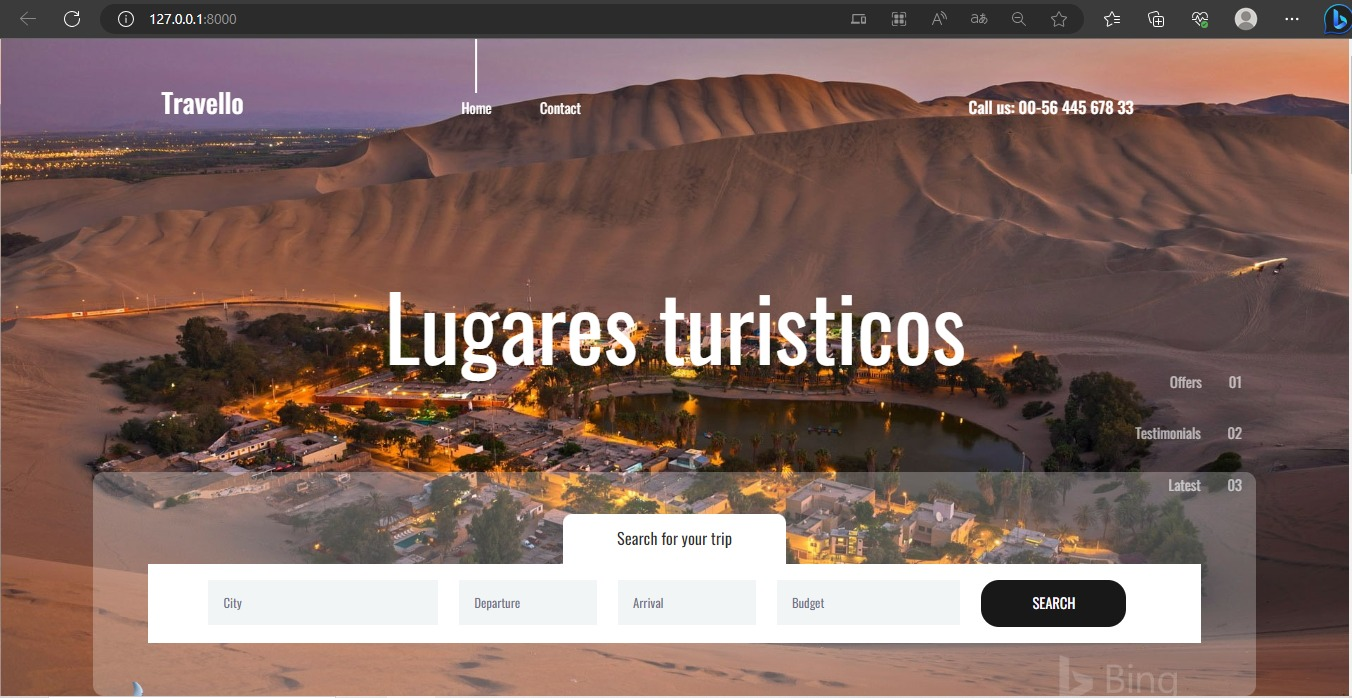
\includegraphics[width=11.2cm]{imagenes/img.jpeg}}}
     
      \item[ ]{\raisebox{-0.2\height}{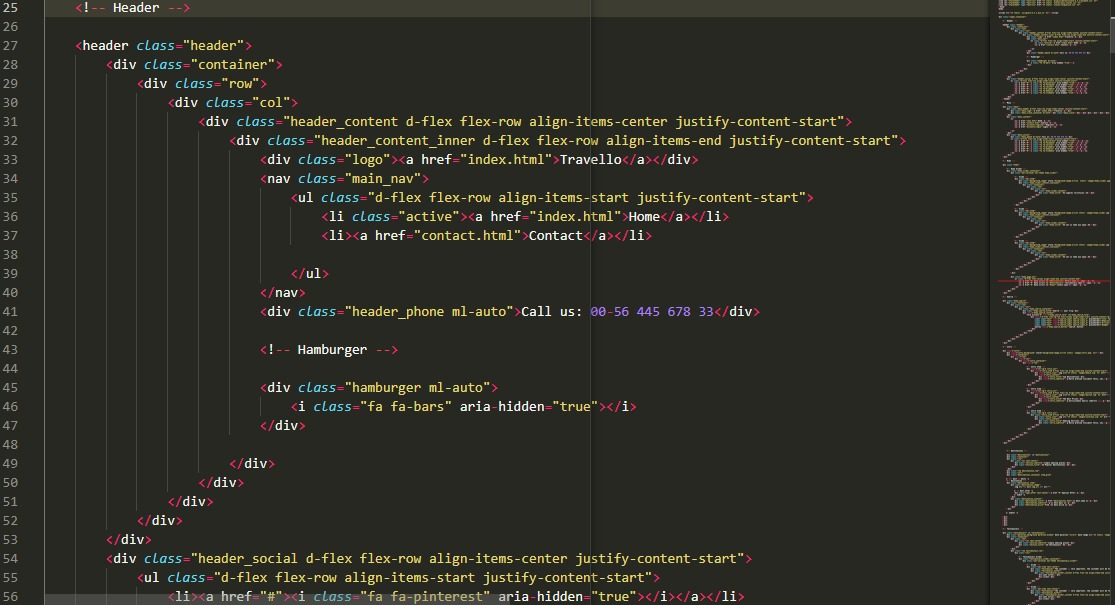
\includegraphics[width=11.2cm]{imagenes/img3.png}}}
      \item Este código crea una estructura básica para el encabezado de un sitio web, que incluye un logotipo, una navegación principal y la información de contacto.
      
      \item[ ]{\raisebox{-0.2\height}{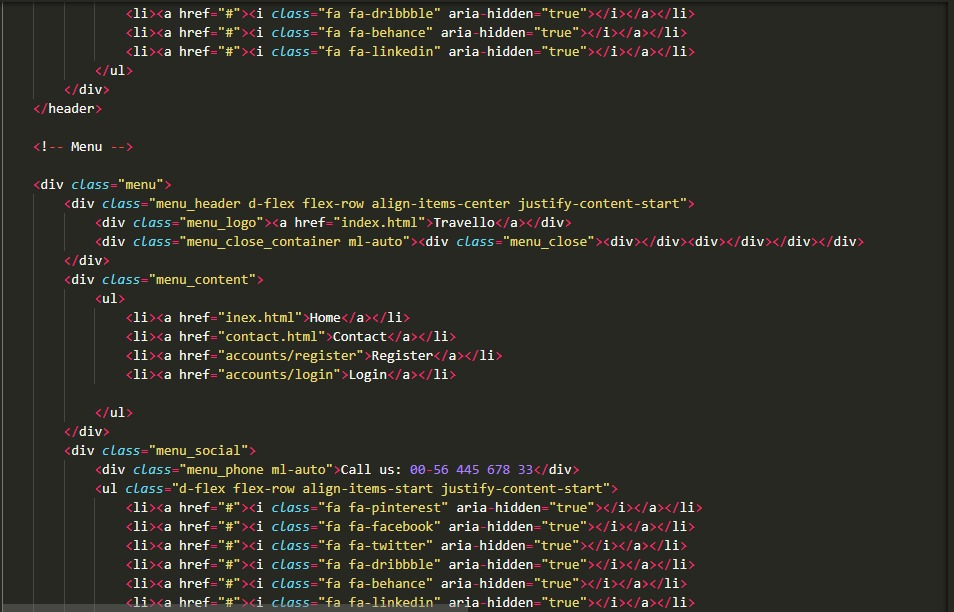
\includegraphics[width=11.2cm]{imagenes/img4.png}}}

     \item En general, este código crea una estructura básica para un encabezado y un menú de un sitio web, con enlaces a las redes sociales y opciones de navegación. El código utiliza la biblioteca de iconos Font Awesome para mostrar íconos junto a los enlaces.
        
      LOGIN
     \item[ ]{\raisebox{-0.2\height}{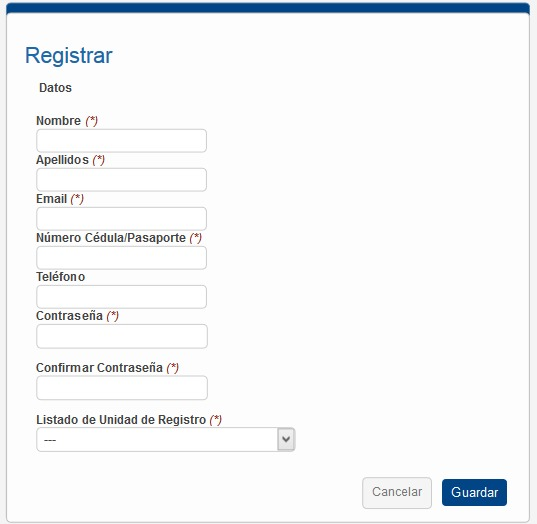
\includegraphics[width=11.2cm]{imagenes/img5.png}}}

     \item Este código crea una página de inicio de sesión básica con un formulario para que los usuarios ingresen sus credenciales y un enlace para registrarse si aún no tienen una cuenta. También incluye la posibilidad de mostrar mensajes o alertas a los usuarios, que pueden ser enviados desde el servidor.

    \item[ ]{\raisebox{-0.2\height}{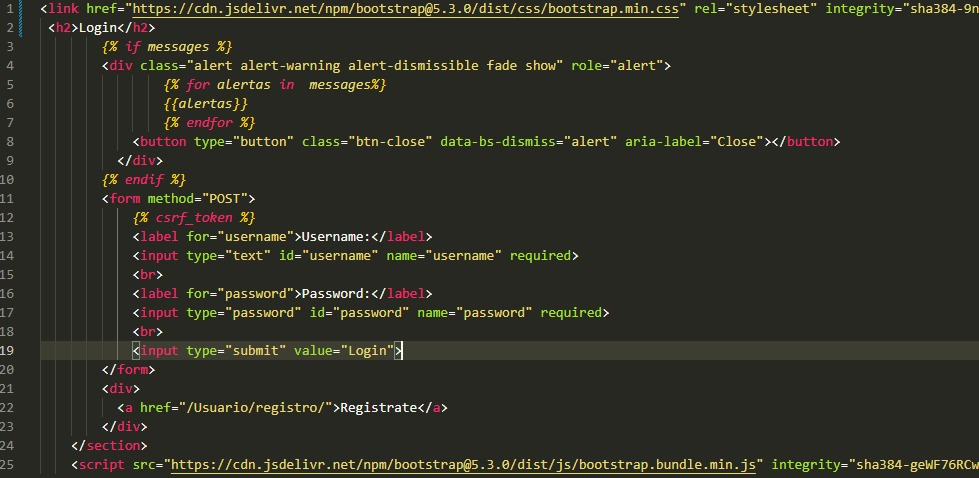
\includegraphics[width=11.2cm]{imagenes/img6.png}}}
 

    \item MAS INFORMACION EN :  https://github.com/MauCausa/Pweb2-Lab-B/tree/main/Lab06-Informe
       
      
           
	\end{itemize}
		
	\section{Equipos, materiales y temas utilizados}
	\begin{itemize}
		
		\item Python 3.11.2.
		\item Git 2.39.2.
		\item Cuenta en GitHub con el correo institucional.
		\item Programación Orientada a Objetos.
		
	\end{itemize}
	
	\section{URL de Repositorio Github}
	\begin{itemize}
		
	\end{itemize}
		
	\begin{itemize}	
		\item Link del repositorio github
        \item \url{https://github.com/MauCausa/Pweb2-Lab-B/tree/main/Lab06-Informe}
	\end{itemize}

\section{Cuestionario}

	\begin{document}
  
   
    \item
    
        
    
        
   \section{} 
  

    
\section{\textcolor{red}{Rúbricas}}
	
	\subsection{\textcolor{red}{Entregable Informe}}
	\begin{table}[H]
		\caption{Tipo de Informe}
		\setlength{\tabcolsep}{0.5em} % for the horizontal padding
		{\renewcommand{\arraystretch}{1.5}% for the vertical padding
		\begin{tabular}{|p{3cm}|p{12cm}|}
			\hline
			\multicolumn{2}{|c|}{\textbf{\textcolor{red}{Informe}}}  \\
			\hline 
			\textbf{\textcolor{red}{Latex}} & \textcolor{blue}{En conclusion este informe esta editado en latex y en formato PDF.}   \\ 
			\hline 
			
			
		\end{tabular}
	}
	\end{table}

\section{Referencias}
\begin{itemize}			
	\item \url{https://www.w3schools.com/python/python_reference.asp}
	\item \url{https://docs.python.org/3/tutorial/}
\end{itemize}	
	
%\clearpage
%\bibliographystyle{apalike}
%\bibliographystyle{IEEEtranN}
%\bibliography{bibliography}
			
\end{document}
	
